\documentclass[12pt, twocolumn]{article}
\usepackage[utf8]{inputenc}
\usepackage[spanish]{babel}
\usepackage{geometry}
\geometry{a4paper,top=0.7in, left=0.5in, right=0.5in, bottom=0.5in}
\usepackage{amsmath}
\usepackage{listings}


\usepackage{graphicx}
\usepackage{float}
\usepackage{url}
\usepackage{booktabs}
\usepackage{chngcntr}
\usepackage{amsfonts}
\usepackage{fancyhdr}
\pagestyle{fancy}
\cfoot{Página \thepage}
\counterwithin*{equation}{subsection}
\newtheorem{theorem}{Propiedad}

\begin{document}
	\title{Medición del ritmo cardíaco por fotopletismografía\\ 
		   \large{\textsc{Métodos Numéricos Avanzados}} \\
		   \normalsize{\textsc{Instituto Tecnológico de Buenos Aires}}}
	\author{
		\textsc{Balaguer}, Pedro \\
		\texttt{55795}
		\and
		\textsc{Benítez}, Julián \\
		\texttt{56283}
		\and
		\textsc{Garrigó}, Mariano \\
		\texttt{54393}
		\and
		\textsc{Perazzo}, Matías \\
		\texttt{55024}
		\and
		\textsc{Saqués}, M. Alejo \\
		\texttt{56047} 
	}
	\date{}
	\maketitle
	
	\begin{abstract}
		
		El ritmo cardíaco $($\textit{Heart Rate}$)$ es un indicador importante del estado fisiológico de una persona. Tradicionalmente, dicho indicador se mide con instrumentos como puede ser un estetoscopio, o bien incluso mediante una simple palpación de las zonas aledañas al corazón.
		
		En este trabajo, se analizó la perspectiva de utilizar una cámara digital con su \textbf{LED} para la determinación del ritmo cardíaco, realizando un análisis de las frecuencias presentes en un vídeo capturado con dicha cámara para la estimación del mencionado indicador.
		
		Se ha constatado que este método es, en efecto, y con el \textit{hardware} apropiado, un método válido para realizar aproximaciones del ritmo cardíaco de un individuo. Si bien sus resultados no deberían ser tenidos en cuenta con propósitos médicos, los datos obtenidos han exhibido que el método analizado puede arrojar resultados con un error relativo de entorno al $5\%$.
		

	\end{abstract}
	
	\paragraph{Palabras clave:} Serie de Fourier, Transformada de Fourier $($continua/discreta$)$, \textit{Fast Fourier Transform}, Filtros de banda.
	
	\section{Transformada de Fourier}
	
	\subsection{Series de Fourier}
	
	\paragraph{} Una serie de Fourier permite descomponer cualquier función periódica en una suma, finita o no, de senos y cosenos.
	
	\begin{align}
		f(x) = \frac{a_{0}}{2} + \sum^{\infty}_{n=1}a_{n}\cos(nx) + \sum^{\infty}_{n=1}b_{n}\sin(nx)
	\end{align}
	
	\paragraph{} Donde $a_{n}$ y $b_{n}$ son los \textbf{coeficientes de Fourier} de la serie de Fourier de la función $f(t)$.
	
	\paragraph{} Con el uso de propiedades trigonométricas, se puede llegar a una expresión reducida:
	
	\begin{align}
		f(x) = \frac{A_{0}}{2} + \sum_{n=1}^{N}A_{n}\cdot\sin(\frac{2\pi nx}{P} + \phi_{n}) \\
		A_{n} = \sqrt{a_{n}^{2}+b_{n}^{2}} \\
		\phi_{n} = \arctan_{2}(a_{n},b_{n})
	\end{align}
	
	\paragraph{} Con $N\ge1$, siendo $f(x)$ integrable en un intervalo $\left[x_{0}, x_{0}+P\right]$. Se puede notar que $A_{n}$ representa el peso del n-ésimo seno dentro de la función periódica $f(x)$.
	
	\subsection{Transformada continua de Fourier}
	
	\paragraph{} La transformada continua de Fourier $($\textbf{TCF}$)$ puede ser entendida como una extensión de las series de Fourier, pero donde el período de la función puede tender a infinito. La transformada de Fourier permite determinar cuál es el \textit{grado de presencia} de cierta frecuencia en una función o señal, es decir, permite transformar un dominio temporal a uno de frecuencias. Nótese que esto no se limita a funciones variables en el tiempo, pero con objetivo de unificar el vocabulario se le llama dominio temporal al dominio de la función original. La transformada de Fourier se define de la siguiente manera:
	
	\begin{align}
		\hat{f}(\xi) = \int_{-\infty}^{\infty} f(x)\cdot\exp^{-2\pi i x\xi} dx
	\end{align}
	
	\paragraph{} Con $x$ perteneciendo al dominio de los tiempos, y $\xi$ al de las frecuencias.
	
	\paragraph{} Utilizando la fórmula de Euler, se ve que la transformada de Fourier puede ser expresada con senos y cosenos:
	
	\begin{align*}
		\exp^{ix}=\cos x + i \sin x
	\end{align*}
	
	\paragraph{} De forma similar a las series de Fourier, donde el valor $A_{n}$ representaba el peso del n-ésimo seno, la transformada de Fourier permite encontrar cada uno de los componentes sinusoidales con frecuencia $\xi$ y su respectivo peso, permitiendo \textit{reconstruir} la función original.
	
	\paragraph{} A continuación sigue un ejemplo ilustrativo del proceso.
	
	\paragraph{} En primer lugar, se considera una función $f(t)$, es decir, con dominio temporal $t \in \left[0,2.5\right]$:
	
	\begin{figure}[H]
		\centering
		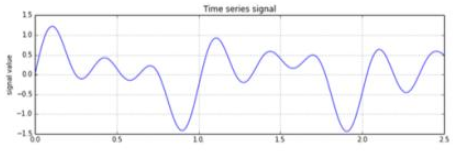
\includegraphics[width=8cm]{ft.png}
		\caption{Alguna función con dominio temporal}
		\label{ft}
	\end{figure}
	
	\paragraph{} Luego, cada punto $($o \textit{vector}$)$, puede proyectarse en un sistema de coordenadas con los ejes \textit{Reales} e \textit{Imaginarios} con una frecuencia $\xi$ dada:
	
	\begin{figure}[H]
		\centering
		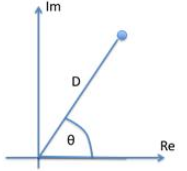
\includegraphics[width=5cm]{imre.png}
		\caption{Ejes coordenados}
		\label{imre}
	\end{figure}
	
	\paragraph{} Con $\Phi=2\pi t\xi$ y $D=f(t)$

	\paragraph{} Proyectando cada punto de $f$ para todo $t$ en el dominio de la muestra, fijando distintas frecuencias $\xi$, obtendríamos, para este ejemplo, los siguientes resultados:
	
	\begin{figure}[H]
		\centering
		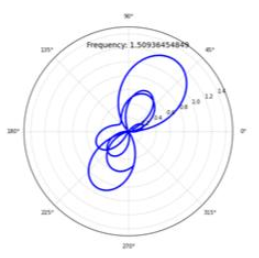
\includegraphics[width=5cm]{f1-5.png}
		\caption{Ejemplo para $\xi = 1.509$ }
		\label{f1-5}
	\end{figure}
	
	\begin{figure}[H]
		\centering
		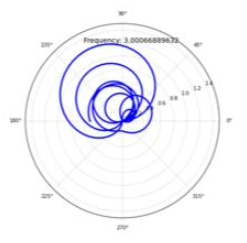
\includegraphics[width=5cm]{f3-0.png}
		\caption{Ejemplo para $\xi = 3.0007$ }
		\label{f3-0}
	\end{figure}
	
	\paragraph{} Las figuras \ref{f1-5} y \ref{f3-0} corresponden a la siguiente expresión para alguna frecuencia $\xi$ dada:
	
	\begin{align}
		f(t)\exp(-2i\pi t \xi)
	\end{align}
	
	\paragraph{}Finalmente, para obtener el peso de la función sinusoidal con frecuencia $\xi$, se suman los módulos de los vectores de la proyección. Luego, se obtiene una función $\hat{f}(\xi)$ que representa el peso de cada frecuencia $\xi$ en la función $f(t)$ dependiente del tiempo.
	
	\subsection{Transformada discreta de Fourier}
	
	\paragraph{} La transformada discreta de Fourier $($\textbf{TDF}$)$ guarda la misma esencia que la continua. Esta transformada permite representar el dominio de las frecuencias de una señal a partir del muestreo de una señal continua cada intervalos de tiempo constantes. La expresión de la \textbf{TDF} es la siguiente:  
	
	\begin{align}
		X_{k} = \sum_{n=0}^{N-1}x_{n}\cdot\exp^{-\frac{2\pi i}{N}k n}
	\end{align}
	
	\paragraph{} Lo cual transforma una secuencia de $N$ números complejos $x_{0},x_{1},\dots,x_{N-1}$, en otra secuencia de sobre el mismo cuerpo $X_{0},X_{1},\dots,X_{N-1}$. Aquí $0\le k\le N-1$. La interpretación es que $\hat{f}(\xi_{k})=X_{k}$.
	
	\paragraph{} Se puede notar que la expresión de la \textbf{TDF} es muy similar a la de la \textbf{TCF}, con la única diferencia de que la primera utiliza una sumatoria en vez de una integral, ya que en este caso se está tratando con una cantidad discreta de valores. Por ende, salvando esta diferencia, la interpretación gráfica del proceso es análogo al caso anterior.
	
	\subsubsection{Algoritmo por fuerza bruta}
	
	\paragraph{} El algoritmo por fuerza bruta es, en esencia, lo que su nombre indica: utilizar la expresión de la \textbf{TDF} exhibida más arriba para realizar el cálculo de la transformada. Esto implica que, por cada $X_{k}$, se realiza una sumatoria sobre $N$ productos, por lo que el orden algorítmico de esta implementación es $O(N^{2})$.
	
	\subsubsection{\textit{Fast Fourier Transform}}
	
	\paragraph{} Una versión mejorada de la implementación de la \textbf{FFT}, propuesta por Cooley y Tukey $($1965$)$, permite reducir el orden computacional a $O(n\cdot log n)$. La idea se basa en el aprovechamiento de las simetrías de $\exp^{-\frac{2\pi i k n}{N}}$ en la expresión de la \textbf{TDF}.
	
	\paragraph{} Sea $W_{N} = \exp^{-\frac{2\pi i}{N}}$. Luego, puede verse que:
	
	\begin{align}
		W_{N}^{kN} = \exp^{-2\pi i k} = 1
	\end{align}
	
	Luego, se tienen las siguientes propiedades:
	
	\begin{theorem}[Simetría conjugada compleja]
		\begin{align*}
			W_{N}^{k(N-n)} = W_{N}^{-kn} = (W_{N}^{kn})^{*}
		\end{align*}
	\end{theorem}
	
	\begin{theorem}[Periodicidad en $n$ y $k$]
		\begin{align*}
			W_{N}^{kn} &= W_{N}^{k(N+n)} \\
			&= W_{N}^{(k+N)n}
		\end{align*}
	\end{theorem}
	
	\paragraph{} La transformada rápida de Fourier se basa en el concepto de \textit{divide and conquer}: asumiendo la cantidad de entradas $N = 2^{m}$ se subdivide el problema en dos de tamaño $\frac{N}{2}$ a partir de los cuales es posible calcular el primero. El enfoque más común es dividir el cálculo de la transformada de Fourier según índices pares e impares:
	
	\begin{align}
		X_{k} &= \sum_{k=0}^{N-1} x_{n}W_{N}^{kn} \\
		&= \sum_{n\quad par}x_{n}W_{N}^{kn} + \sum_{n\quad impar}x_{n}W_{N}^{kn} \\
		&= \sum_{r=0}^{\frac{N}{2}-1} x_{2r}W_{N}^{k2r} + \sum_{r=0}^{\frac{N}{2}-1}x_{2r+1}W_{N}^{k(2r+1)} \\
		&= \sum_{r=0}^{\frac{N}{2}-1}x_{2r}(W_{N}^{2})^{kr} + W_{N}^{k}\sum_{r=0}^{\frac{N}{2}-1}x_{2r+1}(W_{N}^{2})^{kr}
	\end{align}
	
	\paragraph{} Como $W_{N}^{2} = \exp^{-\frac{2\pi i}{N}2} = \exp^{-\frac{2\pi i}{\frac{N}{2}}} = W_{\frac{N}{2}}$.
	
	\paragraph{} Sea $X_{p_{k}}$ la \textbf{TDF} para las muestras pares y $X_{i_{k}}$ para las impares. Esto implica que se pueden calcular de forma independiente $X_{p_{k}}$ y $X_{i_{k}}$, ambas con $\frac{N}{2}$ muestras en vez de $N$, luego combinando los resultados para obtener $X_{k}$.
	
	\paragraph{} Nótese que, gracias a la Propiedad 2, $X_{p_{k+\frac{N}{2}}} = X_{p_{k}}$ $($ídem para $X_{i})$ Luego:
	
	\begin{equation}
	X_{k}=
	\begin{cases}
	X_{p_{k}}+W_{N}^{k}X_{i_{k}}, & \text{si}\ 0\le k< \frac{N}{2} \\
	X_{p_{k-\frac{N}{2}}}+W_{N}^{k}X_{i_{k-\frac{N}{2}}}, & \text{si}\ \frac{N}{2}\le k < N
	\end{cases}
	\end{equation}
	
	\paragraph{} También se puede obtener:
	
	\begin{align*}
		X_{k} = X_{p_{k}} + W_{N}^{k}X_{i_{k}} \\
		X_{k+\frac{N}{2}} = X_{p_{k}} - W_{N}^{k}X_{i_{k}}
	\end{align*}
	
	\paragraph{} A partir de estos resultados se puede realizar un algoritmo recursivo para calcular la \textbf{TDF} con orden computacional $O(n\cdot \log n)$. A continuación, presentamos el pseudo-código de la transformada rápida de Fourier siguiendo este método:
	
	\newpage
	  
	  
	\begin{lstlisting}[frame=single]  % Start your code-block
	
	def FFT(X):
	  N = len(X)
	  if N > 1:
	    even = X[::2]
	    odd = X[1::2]
	    FFT(even)
	    FFT(odd)
	    for k in range(N/2):
	      e = X[k]
	      o = X[k+N/2]
	      w = exp(-2*pi*1j/n)
	      X[k] = e + w * o
	      X[k+N/2] = e - w * o
	  return X
	  
	\end{lstlisting}
	
	
	\section{Método}
	
	\paragraph{} Lo primero a tener cuenta cuando se toman muestras de una señal es el ancho de banda. El latido de un corazón humano promedio se encuentra entre los 60 (1 Hz) y 100 (1.667 Hz) latidos por minuto (ppm o \textit{bpm}) y varía según la edad, el estado físico  y la actividad física que se esté realizando. Según la \textbf{ley de Nyquist}, la frecuencia del muestreo debe ser de por lo menos el doble del valor máximo posible (3.334 Hz) para capturar todo el rango de frecuencias de los latidos sin posibilidad de que exista \textit{aliasing}. Una cámara estándar filma vídeos en al menos 30 fps, es decir, con una frecuencia de al menos 30 Hz. Por ende, se puede decir que la frecuencia de muestreo provista por un \textit{hardware} básico es suficiente para los fines de este trabajo.
	
	\paragraph{} Uno de los primeros análisis que pueden realizarse se vincula con la definición de un área de interés (\textbf{ROI}) para la extracción de datos de cada trama. El objetivo es obtener de cada trama un escalar representativo.  La \textbf{ROI} definida es, a menudo,  un \textit{trade-off} entre la carga computacional y la influencia del ruido en las muestras extraídas. Si su tamaño es muy grande (eventualmente tomando toda la trama), es probable que la onda generada a partir del promedio de los valores en la \textbf{ROI} sea menos sensible al ruido, pero se requerirá un mayor esfuerzo computacional. En cambio, si el tamaño es muy pequeño, el tiempo computacional será menor, pero la podría ser más susceptible al ruido. En la sección de Resultados se analizarán diferentes \textit{ROI} a los efectos de determinar una \textbf{ROI} que busque minimizar tanto el ruido como el tiempo de ejecución del algoritmo.

	\paragraph{} Una vez obtenido el vector de valores representativos de cada trama, se lo centraliza y se aplica \textbf{FFT} para transformar la señal en el dominio del tiempo al de las frecuencias.
	
	\paragraph{} Dado que las frecuencias de interés se encuentran en un rango de los 60 a 100/110 pulsaciones por minuto, se aplica un filtro cuadrado en dicho rango para eliminar frecuencias que no son de interés. Nótese que esto estaría descartando ritmos cardíacos anormales, pero no por ello imposibles.
	
	\paragraph{} Finalmente, se toma el máximo valor del vector de valores en frecuencias. El valor devuelto como aproximación al ritmo cardíaco es su correspondiente coordenada en las abscisas (frecuencias).
	
	\subsection{Colores en la trama}  
	
	\paragraph{} En este análisis, uno de los aspectos a tener en cuenta gira entorno a los colores en la trama. Dichas tramas poseen 3 componentes: R (\textit{red}), G (\textit{green}) y B \textit{blue}. Uno de los inconvenientes hallados se vincula con la captación de determinadas componentes en dispositivos móviles modernos: en algunos casos, se ha notado la completa ausencia de la componente del G (verde) al capturar vídeos por sobre la piel. Se estima que, en estos dispositivos, la cámara realiza correcciones de color que podrían eliminar componentes que serían imperceptibles al ojo humano, como podría ser el caso de los verdes en una imagen donde predominan los rojos. Por ende, y dado que el flujo de la sangre podría generar alteraciones en el nivel de brillo de todas las componentes como un todo, se ha resuelto convertir la trama en colores a \textbf{escala de grises}. En la sección de Resultados se podrá ver que este enfoque genera aproximaciones satisfactorias.
	

	\section{Resultados}
	
	\paragraph{} A continuación, se exhibirán los tiempos de ejecución entre las diferentes implementaciones del algoritmo \textit{fft} realizadas, como así también de los resultados obtenidos a la hora de calcular el ritmo cardíaco de un individuo.
	
	\subsection{Algoritmos \textit{fft}}
	
	\paragraph{} A continuación, se presenta una tabla comparativa de tiempos de ejecución entre la implementación recursiva e iterativa del algoritmo \textit{fft Cooley-Tukey}.
	
	\begin{table}[H]
		\centering
		\begin{tabular}{@{}llll@{}}
			\toprule
			N    & Recursivo & Iterativo & Mejora \\ \midrule
			512  & .009      & .003      & x3     \\
			1024 & .02       & .006      & x3.34  \\
			2048 & .046      & .014      & x3.29  \\
			4096 & .096      & .029      & x3.21  \\
			8192 & .201      & .06       & x3.35  \\ \bottomrule
		\end{tabular}
		\caption{Comparación entre implementaciones de \textit{Cooley-Tukey}}
		\label{fftcmp}
	\end{table}
	
	\paragraph{} Como podrá verse en la Tabla \ref{fftcmp}, la implementación iterativa del algoritmo \textit{Cooley-Tukey} es claramente del mismo orden algorítmico, pero en torno a $3.3$ veces más rápido. Se arguye que la mejora en la \textit{performance} proviene de la eliminación del \textit{overhead} generado por los \textit{stackframes} producidos por la implementación recursiva en cada llamada.
	
	
	\subsection{Mediciones del ritmo cardíaco}
	
	\paragraph{} Se han tomado 5 muestras de un individuo en diferentes partes del cuerpo, variando el uso del \textbf{LED} del dispositivo. Se han tomado 1024 tramas de $640x480$ píxeles, a una frecuencia de muestreo de 30 fps. Se entiende que el dispositivo utilizado (\textit{Samsung Galaxy Note II}) no realiza alteraciones sustanciales sobre las tramas obtenidas. A continuación se describen las áreas del cuerpo y las configuraciones tenidas en cuenta:
	
	\begin{enumerate}
		\item Índice izquierdo $($cubriendo el \textbf{LED} con el mismo$)$,
		\item Pulgar derecho $($sin cubrir el \textbf{LED}$)$,
		\item Antebrazo,
		\item Índice derecho $($sin cubrir el \textbf{LED}$)$,
		\item Índice derecho $($con el \textbf{LED} apagado$)$.
	\end{enumerate}
	
	\paragraph{} Al momento de tomar las capturas, el individuo se encontraba en reposo. Se procuró que el mismo realizara inhalaciones y exhalaciones a intervalos regulares de aproximadamente 2 segundos, instruyéndole que realizara las mismas de manera calma.
	
	\paragraph{} A modo de control, se tomó una serie de muestras del ritmo cardíaco del individuo con mecanismos tradicionales. Para mayor precisión, se utilizó un estetoscopio y se contó durante el lapso de 1 minuto la cantidad de pulsaciones. Los siguientes parámetros describen la muestra:
	
	\begin{itemize}
		\item $N = 14$
		\item $\bar{X} = 78.929$
		\item $\sigma = 4.0089$
	\end{itemize}
	
	\paragraph{} A continuación se exhibirán los resultados utilizando diferentes métodos para obtener un valor escalar que represente el \textit{brillo} de la imagen para un instante dado, tomando una trama en escala de grises. 
	
	\paragraph{} Debe notarse que, en el análisis a continuación, se asume que el rimo cardíaco real permanece constante entre cada una de las muestras tomadas. Dadas las circunstancias en las que se re han realizado las mediciones, esta asunción puede tener un grado alto de validez. Sin embargo, eventuales variaciones podrían influir sobre la precisión de los errores presentados a continuación.
	
	\subsection{Región cuadrada con vértice en el centro}
	
	\paragraph{} Para este caso, se ha tomado una región cuadrada de $30X30$ con vértice en el centro de la imagen. Este caso es el utilizado por la Cátedra en el código de ejemplo.
	
	\begin{table}[H]
		\centering
		\begin{tabular}{@{}lll@{}}
			\toprule
			Muestra & Ppm.   & $|Error|$  \\ \midrule
			1    & 73.815 & 6.93\% \\
			2    & 75.592 & 4.41\% \\
			\textbf{3}    & 86.150 & 9.15\% \\
			4    & 80.854 & 2.44\% \\
			5    & 84.316 & 6.83\% \\ \bottomrule
		\end{tabular}
		\caption{Región $30X30$ con vértice en el centro}
		\label{3030}
	\end{table}
	
	\paragraph{} Como podrá verse en el Cuadro \ref{3030}, la aproximación con menor error relativo al promedio ha sido la de la muestra correspondiendo al dedo índice sin cubrir el \textbf{LED}. Por otro lado, la que mayor error relativo parecería mostrar es el caso del antebrazo.
	
	\subsection{Promedio de toda la imagen}
	
	\paragraph{} En este caso, se han promediado todos los puntos de la imagen en escala de grises.
	
	\begin{table}[H]
		\centering
		\label{my-label}
		\begin{tabular}{@{}lll@{}}
			\toprule
			Muestra & Ppm.   &  $|Error|$    \\ \midrule
			1    & 73.815 & 6.93\%  \\
			2    & 86.139 & 9.13\%  \\
			3    & 87.908 & 11.38\% \\
			4    & 80.853 & 2.44\%  \\
			5    & 59.724 & 32.16\% \\ \bottomrule
		\end{tabular}
		\caption{Promedio de toda la imagen}
		\label{prom}
	\end{table}
	
	\paragraph{} Utilizando el método anterior, el error relativo en la muestra 5 era comparable al de las otras muestras. En el Cuadro \ref{prom}, podrá verse que dicho error, con este método, excede con creces el de las otras muestras. Esto indicaría que utilizar el \textbf{LED} podría ser un requisito indispensable a la hora de aproximar el ritmo cardíaco.
	
	\begin{figure}[H]
		\centering
		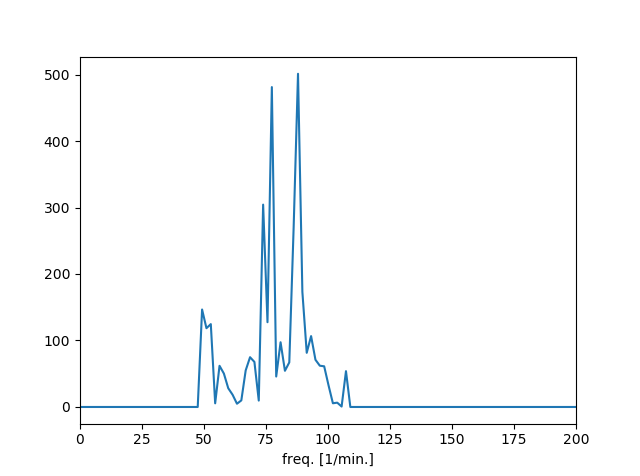
\includegraphics[width=8cm]{sample3_all.png}
		\caption{Muestra 3: proximidad entre picos}
		\label{3prox}
	\end{figure}
	
	\paragraph{} Otro caso cuyo error creció con respecto al obtenido en el método anterior es el de la muestra 3. Sin embargo, como se podrá ver en la Figura \ref{3prox}, existen dos picos de magnitud comparable claramente distinguibles uno del otro. El mayor es, razonablemente, el que corresponde a la frecuencia $87.908$. El que le sigue, corresponde al valor de $77.016$, lo que, de tomarse como valor del ritmo cardíaco, marcaría un $|Error| = 2.48\%$. Esto podría ser absolutamente azaroso, pero la eventual precisión del segundo valor en magnitud suscita curiosidad sobre la perspectiva de poder tomar la frecuencia del segundo mayor pico al tomar la medición en el antebrazo.
	
	\subsection{Región cuadrada con vértice en el centro, interpolando puntos}
	
	\paragraph{} Para este último caso, se ha tomado una región cuadrada de $200X200$ con vértice en el centro de la imagen, interpolando de a $5$ píxeles. El objetivo de esto es maximizar la superficie cubierta, a la vez que se toma una cantidad similar de píxeles que en el primer caso. Dado que se está filmando con la lente inmediatamente sobre la piel, la distancia real entre los píxeles es ínfima. Luego, al interpolar muy probablemente se obtenga una aproximación cercana al verdadero promedio de todos los píxeles de la región.
	
	\begin{table}[H]
		\centering
		\begin{tabular}{@{}lll@{}}
			\toprule
			Muestra & Ppm.   &  $|Error|$   \\ \midrule
			1       & 73.815 & 6.93\%  \\
			2       & 73.834 & 6.90\%  \\
			3       & 87.908 & 11.38\% \\
			4       & 80.853 & 2.44\%  \\
			5       & 59.724 & 32.16\% \\ \bottomrule
		\end{tabular}
		\caption{Interpolando}
		\label{inter}
	\end{table}
	
	\paragraph{} Como podrá verse en la Tabla \ref{inter}, salvo una aparente mejoría en la muestra 2, los valores del $|Error|$ son aproximadamente similares a los del caso anterior. 
	
	\begin{figure}[H]
		\centering
		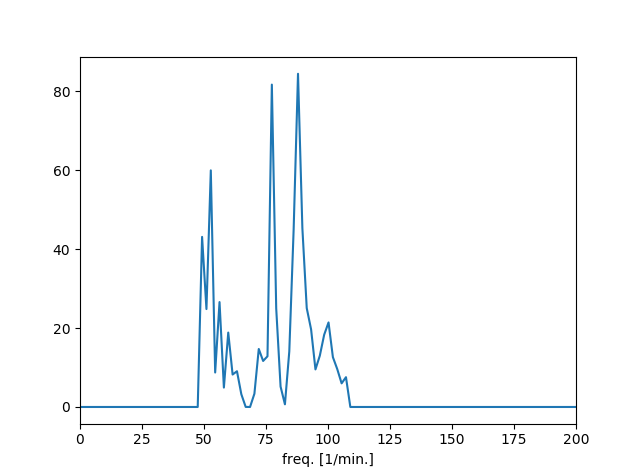
\includegraphics[width=8cm]{sample3-c200_200_5.png}
		\caption{Muestra 3: proximidad entre picos}
		\label{3prox1}
	\end{figure}
	
	\paragraph{} Tal como se ha observado en el método de promediado anterior, en la muestra 3, tras una inspección del gráfico de frecuencias, se observan dos picos de magnitud comparable. En este caso, el valor de la segunda frecuencia más representativa es de $77.419$, lo que representaría un $|Error| = 1.95\%$, el menor de todos los errores relativos obtenidos hasta el momento. 
	
	\subsection{Nueva muestra en el antebrazo}
	
	\paragraph{} En los apartados anteriores, se ha notado una característica particular en la gráfica de frecuencias para los vídeos tomados sobre el antebrazo. Se ha considerado oportuno indagar sobre dicho punto, tomando 2 nuevas mediciones sobre dicha parte del cuerpo del mismo sujeto de pruebas. A continuación se exhiben las gráficas de frecuencias:
	
	\begin{figure}[H]
		\centering
		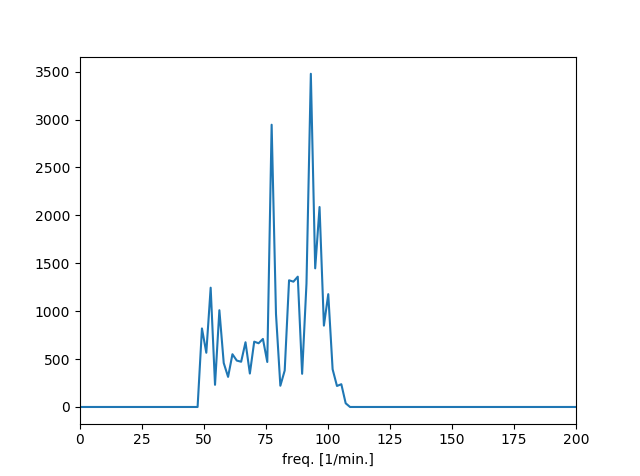
\includegraphics[width=8cm]{sample6-c200_200_5.png}
		\caption{Muestra 6: proximidad entre picos}
		\label{6prox}
	\end{figure}
	
	\paragraph{} Como podrá notarse en la Figura \ref{6prox}, el caso parecería ser idéntico al de la muestra 3: el pico mayor se encuentra en la frecuencia $93.079$, y el que le sigue, en $77.4194$.
	
	\begin{figure}[H]
		\centering
		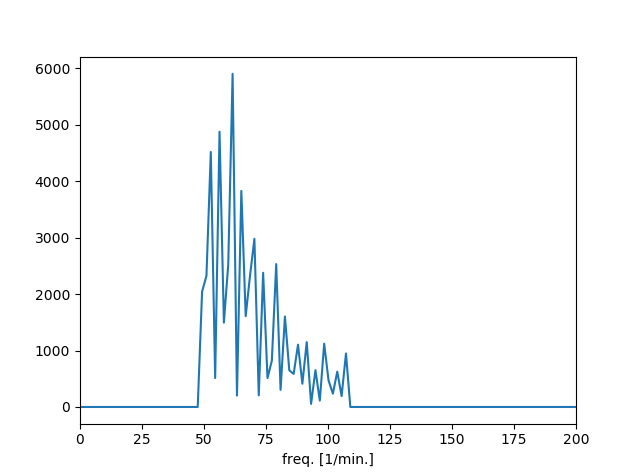
\includegraphics[width=8cm]{sample7-c200_200_5.png}
		\caption{Muestra 6: proximidad entre picos}
		\label{7nprox}
	\end{figure}
	
	\paragraph{} Sin embargo, en la Figura \ref{7nprox}, la estimación obtenida es de $61.535$, y el fenómeno que se observó antes es inexistente. Luego, se podría concluir que lo antes observado responde al azar producto del \textit{ruido} al tomar la filmación. Además, dada la falta de precisión en todas las medidas en las que se utilizó el antebrazo, podría decirse que dicho sector del cuerpo no es apropiada para estimaciones certeras.
	
	\section{Conclusión}
	
	\paragraph{} Se ha determinado que técnicas de fotopletismografía, utilizando cámaras no especializadas, pueden generar aproximaciones razonables al ritmo cardíaco de un individuo.
	
	\paragraph{} Asimismo, se ha descartado la opción de no utilizar una fuente de iluminación externa durante la captura de las tramas a analizar.
	
	\paragraph{} Se ha concluido que, por un lado, no es necesario que la región del cuerpo a analizar se pose sobre el \textbf{LED} del dispositivo. Por otro lado, se ha determinado que es necesario que el grosor del sector a analizar no supere el de un dedo humano. 
	
	\paragraph{} Por último, se ha probado que la extracción de datos desde tramas en \textbf{escala de grises} es un método igual de eficaz al de extraerlas desde tramas en colores. Sobre este punto, se agrega la necesidad de realizar \textbf{FFT} sobre 1 conjunto de datos en vez de 3.
	
	
	
\end{document}